In this chapter the same system models for the robot slide movement are used as presented in \autoref{chap:cbf_1d_static}. Now, however, a dynamic reference is introduced, representing setpoints at a fixed distance to a moving surface such as a beating heart. An new set of states is introduced representing the movement of the beating heart simplified as a sine
\begin{equation}
\dot{x}_{heart} =
\dot{\begin{bmatrix}
x_{h1}\\x_{h2}
\end{bmatrix}} =
\begin{bmatrix}
0 & \omega_h \\ -\omega_h & 0
\end{bmatrix}
\begin{bmatrix}
x_{h1}\\x_{h2}
\end{bmatrix}
\label{eq:beating_heart_sine}
\end{equation}
where $x_{h1}$ is the position of a point on the surface of the heart and $x_{h2}$ is the velocity of the point.
Here $\omega_h$ represents the frequency of the heart, and with an average heartbeat period of 1.1\,s \citep{bib:heart_berkeley}, $\omega_h$ is set to be $2\pi/1.1$. In \autoref{fig:1stordersys_dynamiclimits} the moving surface of the heart is plotted over time, offset to an axis of oscillation in -6\,cm relative to the slide position. This curve marks the boundary to the unsafe region below it, and crossing this curve (from the safe region above it) corresponds to penetrating the heart surface with the surgical instrument tip. Note that the flexibility of the surface of the heart, at contact with the rigid tool, is not considered in the scope of this thesis. 

\begin{figure}[htbp]
	\centering
	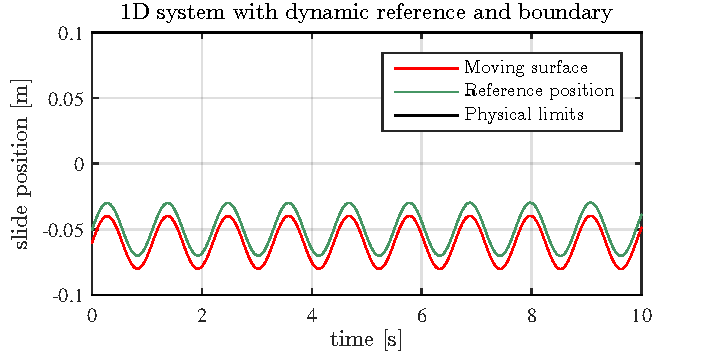
\includegraphics[width=0.6\textwidth]{1stordersys_dynamiclimits.pdf}
	\caption{Example of a moving surface representing the heart, marking the boundary to the unsafe region $\mathcal{X}_u$. A reference is set within the safe region as a fixed distance to the surface of the beating heart.}
	\label{fig:1stordersys_dynamiclimits}
\end{figure}

In \autoref{fig:1stordersys_dynamiclimits} a sine amplitude of 2\,cm is used and a reference defined as the 1D vector $d_{ref}=x_1-x_{h1}$, representing the robot tool distance to the point on the surface of the heart, is set to 1\,cm. This reference difference can be picked as any nonnegative value still allowing the slide position to stay within its (upper) physical limit.
The reference for the robot tool position will in the following be defined as this positive difference in position, i.e.
\begin{equation}
u(t) = \bar{N}(x_{h1}(t)+d_{ref})-kx(t)
\end{equation}
where $x$ here is the state vector of the 1D surgical robot system. \textcolor{red}{Or should it be $-k_1x_1$ no matter the order of the system?}
The dynamic surface representing the heart also put forth new requirements to the safety controller, as the boundary between the safe and unsafe regions $\mathcal{X}_0$ and $\mathcal{X}_u$ is now moving concurrently with the heart surface. This requires the construction of barrier certificates that are functions of robot state as well as the dynamic surface position.



\section{Safe Controller Design for First Order System}
\textcolor{red}{introduce}

\subsection{Setting up the Closed-Loop System and Designing the Linear Controller}
An augmented state-space model including the dynamics of the robot tool from \autoref{eq:1storder_1D_ss} as well as the beating heart from \autoref{eq:beating_heart_sine}, is set up for the closed-loop first order system
\begin{equation}
\dot{\begin{bmatrix}
	x_1\\x_{h1}\\x_{h2}
	\end{bmatrix}} =
\begin{bmatrix}
-(1+k)/\tau & \bar{N}/\tau & 0\\0 & 0 & \omega_h \\ 0 & -\omega_h & 0
\end{bmatrix}
\begin{bmatrix}
x_1\\x_{h1}\\x_{h2}
\end{bmatrix}+ 
\begin{bmatrix}
\bar{N}/\tau \\ 0 \\ 0
\end{bmatrix}
d_{ref}
\end{equation}
\begin{tabular}{rl}
where &\\
$\tau$ & is the time constant of the first order system $\tau=0.11$\,s as given in \autoref{sec:model_slide}\\
$k$ & is the linear system controller designed according to \autoref{eq:K_1}\\
$\bar{N}$ & is the system gain found according to \autoref{eq:barm_1}
\end{tabular}\\

Can also be written with the reference distance $d_{ref}$ as part of the state, with no dynamics indicating it is a fixed value:
\begin{equation}
f_{cl}(x)=\dot{\begin{bmatrix}
	x_1\\x_{h1}\\x_{h2}\\d_{ref}
	\end{bmatrix}} =
\underbrace{\underbrace{\begin{bmatrix}
		-1/\tau & 0 & 0 & 0\\0 & 0 & \omega_h & 0 \\ 0 & -\omega_h & 0 & 0 \\ 0& 0 & 0 & 0
		\end{bmatrix}}_{A}
	\begin{bmatrix}
	x_1\\x_{h1}\\x_{h2}\\d_{ref}
	\end{bmatrix}}_{f(x)}+ 
\underbrace{\underbrace{\begin{bmatrix}
		1/\tau \\ 0 \\ 0 \\ 0
		\end{bmatrix}}_{B}}_{g(x)}
\underbrace{\underbrace{\begin{bmatrix}
		-k & \bar{N} & 0 & \bar{N}
		\end{bmatrix}}_{K}
	\begin{bmatrix}
	x_1\\x_{h1}\\x_{h2}\\d_{ref}
	\end{bmatrix}}_{u}
\end{equation}

\textcolor{red}{Should we design a $k$ that is slower conforming with what is found to be implementable?}

\subsection{Constructing a Barrier Function}
As mentioned, a barrier certificate for this system with a zero level set at the surface of the heart, comprises moving boundaries and hence should be a function of both robot and heart position. According to \autoref{def:safety} a $B(x_1,x_{h1})$ should be constructed with unsafe region $\mathcal{X}_u$ below the surface of the heart, i.e. such that $B(x_1,x_{h1})$ is positive if $x_1<x_{h1}$ and negative otherwise. The very simplest function satisfying this requirement is a function
\begin{equation}
B_0(x_1,x_{h1})= c(x_{h1}-x_1)
\end{equation}
with a positive constant $c>0$. This would result in the Lie derivatives % $L_{f_{cl}}B_0(x)$
\begin{subequations}
\begin{align}
L_fB_0(x) &= \frac{dB_0(x)}{dx}f(x) =
\begin{bmatrix}
-c & c & 0 & 0
\end{bmatrix}
\begin{bmatrix}
-x_1/\tau\\
\omega_h x_{h2} \\
-\omega_h x_{h1} \\
0
\end{bmatrix}=
c\left(\omega_h x_{h2} + \frac{ x_1}{\tau}\right)\\
L_gB_0(x) &= \frac{dB(x)}{dx}g(x) =
\begin{bmatrix}
-c & c & 0 & 0
\end{bmatrix}
\begin{bmatrix}
1/\tau\\
0 \\ 0 \\ 0
\end{bmatrix}=
\frac{-c}{\tau}\\
L_{f_{cl}}B_0(x) & 
%=\frac{dB_0(x)}{dx}f_{cl}(x) 
= L_fB_0(x)+L_gB_0(x)u = 
%\begin{bmatrix}
%	-c & c & 0 & 0
%\end{bmatrix}
%\begin{bmatrix}
%\frac{\bar{N}(x_{h1}+d_{ref})-(1+k) x_1}{\tau} \\
%\omega_h x_{h2} \\
%-\omega_h x_{h1}
%\end{bmatrix}=
c\left(\omega_h x_{h2} - \frac{\bar{N}(x_{h1} + d_{ref})-(1+k) x_1}{\tau}\right)
\end{align}
\end{subequations}
The Lie derivative $L_{f_{cl}}B_0(x)$ (with the heart sine placed as in \autoref{fig:1stordersys_dynamiclimits}) should be negative for the intersection of  $x_1\in[-0.1,0.1]$, $x_{h1}\in [-0.08,-0.04]$ and $x_{h2}\in [-0.02,0.02]$. We thus require that (recall from \autoref{eq:barm_1} that $\bar{N}=K+1$ for the present first order system)
\begin{align}
\omega_h x_{h2} &< \frac{\bar{N}(x_{h1} + d_{ref})-(1+k) x_1}{\tau} = \frac{1+k}{\tau}(x_{h1} + d_{ref}-x_1)\nonumber\\
\omega_h x_{h2} \frac{\tau}{1+k} &< x_{h1} + d_{ref}-x_1
\end{align}
With the largest positive value of $x_{h2}=0.02$\,m and the same controller $K=9$ is used as in \autoref{eq:K_1}, the left-hand expression attains a largest value of 0.00126\,m, requiring that the error between the robot tool position and the reference position always be slightly larger than a millimeter. 
%2*pi/1.1*0.02/(10/0.11)
%0.001256637061436
Obviously this barrier function is not valid, and a different function is opted for.

According to \cite{bib:org_control} a barrier certificate might be found iteratively by using $B_0(x)$ in the construction of a barrier certificate on the form
\begin{equation}
B(x) = 
\begin{cases}
B_0(x) & \text{if}\quad L_fB_0(x) \leq -\beta\\
B_0(x)+\alpha(L_fB_0(x)+\beta)^2 & \text{if}\quad L_fB_0(x)>-\beta 
\end{cases}
\end{equation}
where $\alpha>0$, $\beta>0$ are parameters to be determined. For the presented system this gives the barrier candidate function 
\begin{equation}
B(x) = 
\begin{cases}
c(x_{h1}-x_1) & \text{if}\quad c\left(\omega_h x_{h2} +  x_1/\tau\right) \leq -\beta\\
c(x_{h1}-x_1)+\alpha(c\left(\omega_h x_{h2} +  x_1/\tau\right)+\beta)^2 & \text{if}\quad c\left(\omega_h x_{h2} +  x_1/\tau\right)>-\beta 
\end{cases}
\end{equation}
\textcolor{red}{The constant $c$ is unimportant. Set $c=1$.  In the example in \citep{bib:org_control} they chose $\alpha=1/20$ and $\beta=1$, giving}
\begin{equation}
B(x) = 
\begin{cases}
x_{h1}-x_1 & \text{if}\quad x_1 \leq -0.11-0.2\pi x_{h2}\\
x_{h1}-x_1+\dfrac{1}{20}\left(\dfrac{0.2\pi\,\, x_{h2} +   x_1}{0.11}+1\right)^2 & \text{if}\quad x_1 > -0.11-0.2\pi x_{h2} 
\end{cases}
\end{equation}
\textcolor{red}{Need to test this!}


\section{Safe Controller Design for Second Order System}
\textcolor{red}{introduce}

\subsection{Setting up the Closed-Loop System and Designing the Linear Controller}
As for the first order system, the second order system in \autoref{eq:2ndorder_1D_ss} is augmented with the dynamics of the beating heart and with the reference given as a fixed distance from the surface of the beating heart
\begin{equation}
\dot{\begin{bmatrix}
x_1\\x_2\\x_{h1}\\x_{h2}
\end{bmatrix}} = \begin{bmatrix}
0 & 1 & 0 & 0\\
-\omega_n^2(1+k_1)  & -2\zeta \omega_n-\omega_n^2 k_2  & \omega_n^2\bar{N} & 0\\
0 & 0 & 0 & \omega_h \\
0 & 0 & -\omega_h & 0
\end{bmatrix}\begin{bmatrix}
x_1\\x_2\\x_{h1}\\x_{h2}
\end{bmatrix} + \begin{bmatrix}
0\\\omega_n^2\bar{N} \\ 0 \\ 0
\end{bmatrix}d_{ref}
\end{equation}
\begin{tabular}{rl}
where &\\
$\omega_n$ & is the natural frequency of the second order system $\omega_n=17$\,rad/s as given in \autoref{sec:model_slide}\\
$\zeta$ & is the damping ratio of the second order system $\zeta=0.05$ as given in \autoref{sec:model_slide}\\
$[k_1\,\,\,k_2]$ & is the linear system controller designed according to \autoref{eq:K_2}\\
$\bar{N}$ & is the system gain found according to \autoref{eq:Nbar_2}
\end{tabular}\\


Can also be written on augmented form where the reference is part of the state
\begin{equation}
\dot{\begin{bmatrix}
	x_1\\x_2\\x_{h1}\\x_{h2}\\d_{ref}
	\end{bmatrix}} = 
\underbrace{\underbrace{\begin{bmatrix}
		0 & 1 & 0 & 0 & 0\\
		-\omega_n^2  & -2\zeta \omega_n  & 0 & 0 & 0\\
		0 & 0 & 0 & \omega_h & 0\\
		0 & 0 & -\omega_h & 0 & 0\\
		0 & 0 & 0 & 0 & 0
		\end{bmatrix}}_{A}
	\begin{bmatrix}
	x_1\\x_2\\x_{h1}\\x_{h2}\\d_{ref}
	\end{bmatrix}}_{f(x)} + 
\underbrace{\underbrace{\begin{bmatrix}
		0\\\omega_n^2 \\ 0 \\ 0 \\ 0
		\end{bmatrix}}_{B}}_{g(x)}
\underbrace{\underbrace{\begin{bmatrix}
		-k_1 & -k_2 & \bar{N} & 0 & \bar{N}
		\end{bmatrix}}_{K}
	\begin{bmatrix}
	x_1\\x_2\\x_{h1}\\x_{h2}\\d_{ref}
	\end{bmatrix}}_{u}
\end{equation}
